\documentclass[11pt]{article}

\title{Project}
\usepackage{fullpage}
\usepackage{epsfig} 
\pagestyle{empty}
\begin{document}

\section*{Principles of Cyber-Physical Systems\\
Project: Modeling of Collision Avodiance}

\subsection*{Problem}
The goal of this project is to design an aircraft controller that navigates the aircraft from source to destination while ensuring that it does not collide with other aircraft in its path. 
The controller gets information about the current location and the target location of the aircraft. 
Further, it receives messages from aircraft in its vicinity and uses this information to navigate the aircraft and avoid collision with other aircraft. 

In this project, we look at a simplified controller design problem as follows. 
\begin{enumerate}
\item The aircraft can fly in a 2-D plane. Its source and destination are integer-valued points in the plane.
\item The aircraft flies with a constant velocity $v = 1$ km/minute along either X-axis or Y-axis. 
\item The aircraft controller can update direction of flight every $k = 1$ minutes. Note that, it can decide to either fly straight or rotate left or right by 90 degrees but not turn back. 
\item At the beginning of every $k = 1$ minutes, 
\begin{itemize}
\item The controller can exchange messages with any aircraft in a square region with side length $2q = 4$ km (communication zone) in the vicinity of the aircraft as shown in figure below
\item Based on the messages received and the current state of the aircraft, the controller can update the direction of flight.
%\item The direction of flight initially is along positive X axis, which can be updated by the controller at time $t = 0$ minutes. 
\end{itemize}
\item {\bf Collision Avoidance}: Each aircraft has a square region with side length $2d = 1$ km (danger zone) around it such that no aircraft should enter this region at any time during the flight as shown in figure below. 
\item The source locations are distinct locations for different aircraft. 
\item Once an aircraft reaches its destination, it is no longer a threat and collision avoidance is not required for this aircraft. Also, the aircraft stops sending messages to the other aircraft in its vicinity. 
\end{enumerate}
\centerline{
 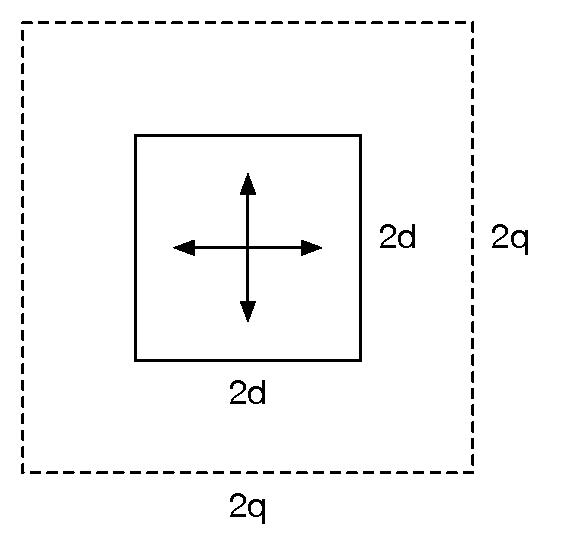
\includegraphics[scale=0.5]{figure.pdf}
}

Further, we assume that the airspace consists only of two aircraft that start at time $t = 0$. 
The goal here is to design a controller (same algorithm for both aircraft) that ensures that each aircraft reaches its destination in as small time as possible while ensuring collision avoidance. 
In the problem, the sources and destinations for aircraft are provided as parameters and the designed controller should work with all such source-destination pairs. 

\subsection*{Project Details}
The project is split into two phases
\begin{itemize}
\item Phase I : Model Design\\
In this phase, a report must be submitted with the following details
\begin{itemize}
	\item Input-output specification: Specify the inputs and outputs of the controller
	\item Requirements: Specify the requirements that the controller must satisfy. 
	\item Design of a \emph{simple} controller: Design an algorithm for a simple controller that ensures that the aircraft reach their destination. 
		The algorithm should be precise and clearly specify how the output of the controller is computed. 
	\item Design of the \emph{complete} controller: Design an algorithm for the controller that ensures that the aircraft reach their destination as well as avoids collision with other aircraft. 
		The algorithm should be precise and clearly specify how the output of the controller is computed.  
		Also, the content of the messages exchanged between the aircraft should be clearly specified. 
	\item Proof of correctness: Show that the designed controller ensures collision avoidance and also that the aircraft reaches its destination. The proof can be informal but must explain why the algorithm for the complete controller is correct. 
\end{itemize}

\item Phase II : Model Implementation\\
In this phase, the controller must be implemented in Matlab. 
\begin{itemize}
	\item Skeleton code to run the simulation and view the trajectories of aircraft will be provided. Details can be found in {\tt Readme.txt} along with code. 
	\item Implement the controller designed in first phase and a safety monitor to check for collision avoidance. Sample implementations are provided in the skeleton code. 
\end{itemize}
\item \emph{Optional:} Design a controller when the airspace consists of three aircraft. 
\end{itemize}

\subsection*{Additional Files}
\begin{enumerate}
\item
The directory Description contains the LaTeX source of this description.
\item
The directory code contain Matlab files of skeleton code (see Readme.txt)
\item
The directory safetyMonitor contains Matlab files that can be used to check correctness of the controller designed by the students.
\end{enumerate}


\end{document}

